\documentclass[11pt]{article}
\usepackage[english]{babel}
\usepackage{amsmath,amssymb,amsfonts}
\usepackage{fullpage}
\usepackage{hyperref}
\usepackage{float}
\usepackage{xcolor}
\usepackage{booktabs}
\usepackage{graphicx}
\usepackage{listings}
\usepackage{titlesec}
\usepackage{fvextra}
% Disable paragraph indentation
\setlength{\parindent}{0pt}%
\setlength{\parskip}{\baselineskip}%
\titleformat{\section}{\large\bfseries}{\thesection}{1em}{}

\lstset{
  language=Python,                 % Set language to Python
  basicstyle=\ttfamily\footnotesize, % Set font and size
  keywordstyle=\color{blue},       % Keywords in blue
  stringstyle=\color{red},         % Strings in red
  commentstyle=\color{green!50!black}, % Comments in green
  backgroundcolor=\color{yellow!10}, % Light gray background
  frame=single,                    % Frame around the code
  numbers=left,                    % Line numbers on the left
  numberstyle=\tiny\color{gray},   % Style for line numbers
  tabsize=6,                       % Set tab width
  showstringspaces=false,           % Hide whitespace symbols
  captionpos=b                     % Caption at the bottom
}

\begin{document}
\title{Assignment3 - DD2424}
\author{Silpa Soni Nallacheruvu}
\date{}
\maketitle

\section*{Gradient Check}

To verify the correctness of my analytical gradient computations for my three-layer ConvNet, I implemented a comparison against the provided debug data for the gradients and other available variables. The relative mean and max errors were computed for each layer's weights, biases and more:
\begin{table}[h!]
  \centering
  \begin{tabular}{|l|c|c|}
  \hline
  \textbf{Comparison} & \textbf{Max Difference} & \textbf{Mean Difference} \\
  \hline
  X\_conv Vs conv\_outputs           & $0.0$                        & $0.0$ \\
  conv\_outputs\_mat Vs conv\_outputs\_flat & $1.70 \times 10^{-13}$       & $6.83 \times 10^{-16}$ \\
  conv\_flat                         & $0.0$                        & $0.0$  \\
  h                                  & $0.0$                        & $0.0$  \\
  p                                  & $6.76 \times 10^{-16}$       & $5.01 \times 10^{-17}$ \\
  Fs\_flat                           & $1.64 \times 10^{-14}$       & $8.45 \times 10^{-16}$ \\
  W1                                 & $4.50 \times 10^{-14}$       & $2.03 \times 10^{-16}$ \\
  W2                                 & $4.51 \times 10^{-15}$       & $1.25 \times 10^{-16}$ \\
  b1                                 & $4.22 \times 10^{-16}$       & $4.22 \times 10^{-17}$ \\
  b2                                 & $1.31 \times 10^{-15}$       & $2.34 \times 10^{-16}$ \\
  \hline
  \end{tabular}
  \caption{Numerical comparison of intermediate computations and gradients.}
  \end{table}

As the mean and max difference between provided debug values and my computed values are insignificant, I conclude that my implementation is bug free.

\section*{Initial Three layer ConvNet}

The initial three-layer ConvNet was implemented with the following architecture:
\begin{itemize}
  \item Convolutional layer with 32 filters of size 3x3, stride 1, and padding 1.
  \item ReLU activation function.
  \item Max pooling layer with a pool size of 2x2 and stride 2.
  \item Fully connected layer with 128 units.
  \item ReLU activation function.
  \item Output layer with softmax activation for classification.
\end{itemize}

The network was trained on the CIFAR-10 dataset with training size of 49,000 images and validation size of 1,000 images. The short training runs with cyclic learning rates from Assignment2 was applied with a minimum learning rate of 1e-5 and a maximum learning rate of 1e-1 for three cycles with constant steps of 800. 

The model with Network architecture 2 ($f=4, nf=10, nh=50$) achieved a final validation accuracy of $56.1\%$ and test accuracy of $55.88\%$. The training time was reported as $13.07$ seconds.

Next, we compare the final test accuracy and training time of all four network architectures with varying f anf nf values with short training runs:

\begin{figure}[H]
    \centering
    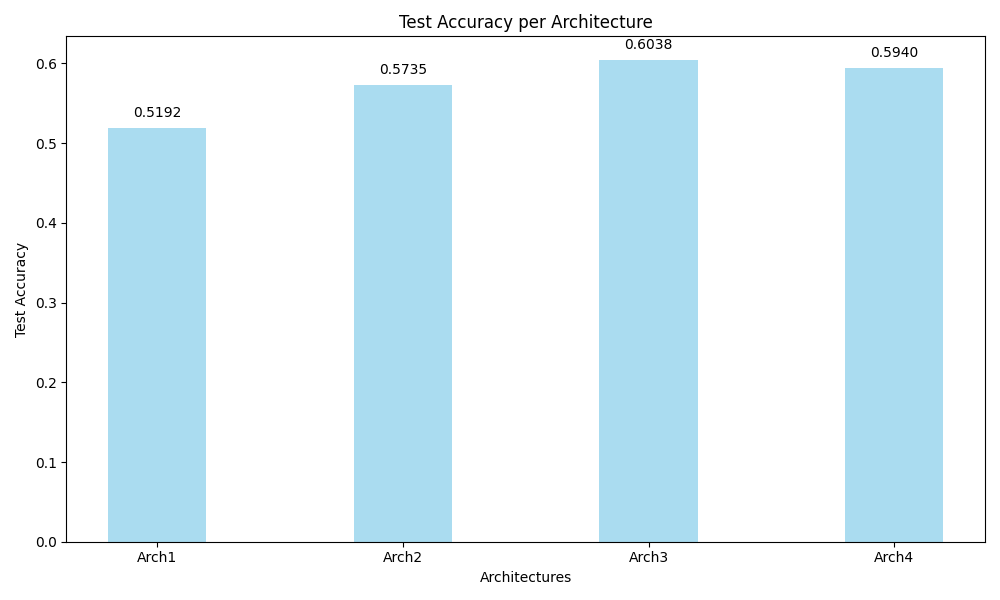
\includegraphics[width=0.8\textwidth]{results/architecture_test_accuracy.png}
    \caption{Comparison of final test accuracy for different network architectures.}
    \label{fig:network_architecture_acc_comparison}
\end{figure}

\begin{figure}[H]
  \centering
  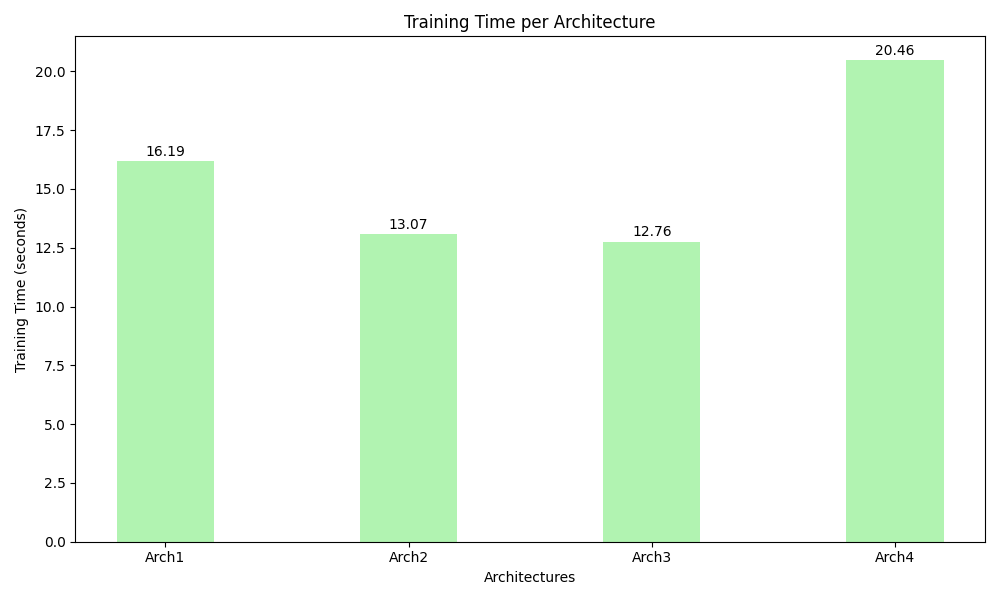
\includegraphics[width=0.8\textwidth]{results/architecture_training_time.png}
  \caption{Comparison of total training time for different network architectures.}
  \label{fig:network_architecture_training_time_comparison}
\end{figure}




\end{document}